\scanpage{82}
% @0 upper right
\mspage{- 23 -}
% @1–2 underlying sheaf
La propriété de $C$-acyclicité ne dépend que du faisceau abélien sous-jacent (2.6).

% @3–5 restriction
Soient $C$ et $C'$ deux sites et $u:C\mathrel{\relbar\joinrel\handwritten{\rightarrow}}C'$ un foncteur continu (3.2.2.III). Il n'est pas vrai, en général, que la restriction à $C''$ d'un faisceau $C'$-acyclique soit $C$-acyclique.

% @6–7 proposition
\noindent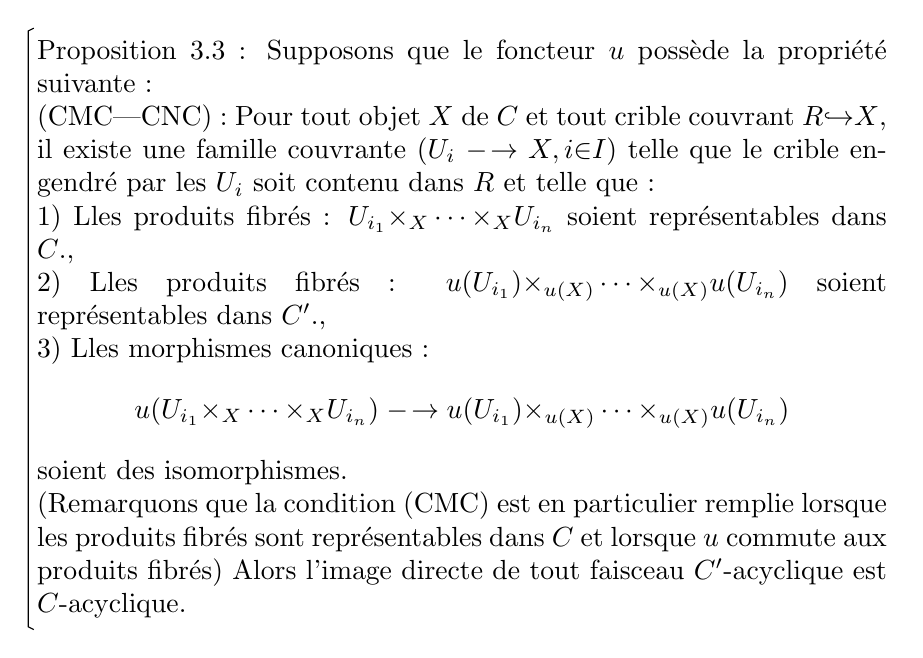
\begin{tikzpicture}
\node[inner sep=3pt] (prop) {\begin{minipage}{.89\linewidth}
\uline{Proposition 3.3} : Supposons que le foncteur $u$ possède la propriété suivante :

% @8–10 covering condition
(\unsure{CMC|CNC}) : Pour tout objet $X$ de $C$ et tout crible couvrant $R\handwritten{\hookrightarrow}X$, il existe une famille couvrante $(U_i\mathrel{\relbar\joinrel\handwritten{\rightarrow}}X,i\handwritten{\in} I)$ tel\handwritten{le} que le crible engendré par les $U_i$ soit contenu dans $R$ et telle que :

% @11–12 first product
1) \deleted{L}\handwritten{l}e\handwritten{s} produits fibrés : $U_{i_1}\handwritten{\times}_X\cdots\handwritten{\times}_X U_{i_n}$ soient représentables dans $C$\deleted{.}\handwritten{,}

% @13–14 second product
2) \deleted{L}\handwritten{l}es produits fibrés : $u(U_{i_1})\handwritten{\times}_{u(X)}\cdots\handwritten{\times}_{u(X)}u(U_{i_n})$ soient représentables dans $C'$\deleted{.}\handwritten{,}

% @15–17 morphisms
3) \deleted{L}\handwritten{l}es morphismes canoniques :
\[
 u(U_{i_1}\handwritten{\times}_X\cdots\handwritten{\times}_X U_{i_n})\mathrel{\relbar\joinrel\handwritten{\rightarrow}}
 u(U_{i_1})\handwritten{\times}_{u(X)}\cdots\handwritten{\times}_{u(X)}u(U_{i_n})
\]
soient des isomorphismes.

% @18–21 conclusion
(Remarquons que la condition (CMC) est en particulier remplie lorsque les produits fibrés sont représentables dans $C$ et lorsque $u$ commute aux produits fibrés) Alors l'image directe de tout faisceau $C'$-acyclique est $C$-acyclique.
\end{minipage}};
\handwritten{\draw (prop.north west) ++(2pt,1pt) -- (prop.north west) -- (prop.south west) -- ++(2pt,-1pt);}
\end{tikzpicture}
% @22 foot
\hfill \ldots/\ldots
% archive sheet number: 81

